\documentclass[11pt, a4paper]{article}

\usepackage[top = 0.7 in, bottom = 0.7 in, left = 0.7 in, right = 0.7 in ]{geometry}

\usepackage{amsmath, amssymb, amsfonts}
\usepackage{enumerate}
\usepackage{array}
\usepackage{multirow}
\usepackage{dingbat}
\usepackage{fontawesome5}
\usepackage{tasks}
\usepackage{bbding}
\usepackage{xcolor}
\usepackage{graphicx}
\usepackage{hyperref}

\definecolor{col1}{HTML}{e75e05}
\definecolor{col2}{HTML}{d30bb1}

\title{MSMS - 105}
\author{Ananda Biswas}
\date{}


\begin{document}

\maketitle

\begin{center}
\textbf{Assignment 04}
\end{center}


\OrnamentDiamondSolid \hspace{0.5cm} \textcolor{blue}{\textbf{Objective :}} To create animated plots to get visual illustrations of different aspects of  \textbf{Matrix Multiplication}. \\

\faArrowAltCircleRight[regular] \textcolor{col1}{\textbf{\textit{Theory}}} : Essence of matrix multiplication is best understood when it is seen as a linear transformation. The geometric interpretation of matrix multiplication provides insights into how matrices transform vectors of a vector space. \\

\hspace{1cm} In the following we shall see different aspects of matrix multiplication. For best visualization experience, we have considered $\mathbb{R}^2$ as our vector space. In each of the illustrations, we have taken 100 vectors originated at $(0, 0)$ and their tips together form a circle. We shall see how matrix multiplication changes the vectors and consequently the circular shape. \\

\begin{figure}[h]
\centering
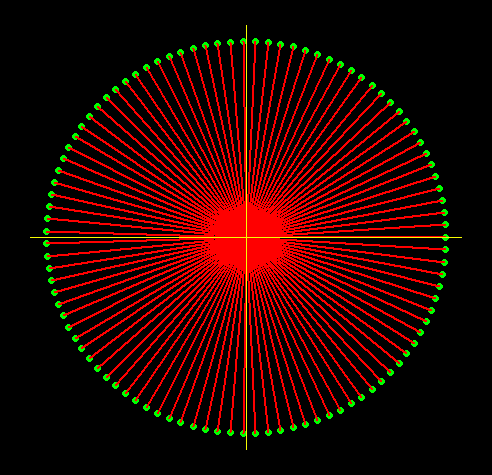
\includegraphics[scale = 0.35]{01}
\end{figure}

\href{https://github.com/sakunisgithub/R-programming/blob/master/msc_sem_1_practicals/mahaveer_sir_assignments/assignment_04/initial_vectors.R}{\textcolor{blue}{\textbf{Program to create the above plot is here.}}} \\

\smallpencil \hspace{0.2cm} \textcolor{col2}{\textbf{\textit{Scaling}}} : Pre-multiplying any vector $ \begin{bmatrix} a \\ b \end{bmatrix} $ $\in$ $\mathbb{R}^2$ by 
  $ \begin{bmatrix} 
      s_x & 0 \\
      0 & s_y 
    \end{bmatrix} $ scales the vector by a factor of $s_x$ along $x-$axis and by a factor of $s_y$ along $y-$axis. \\

Here we pre-multiply $ \begin{bmatrix} 
      1 & 0 \\
      0 & 2 
    \end{bmatrix} $ with initial 100 vectors. \\
    
\faArrowAltCircleRight[regular] \textcolor{col1}{\textbf{\textit{Visualization}}} : \href{https://github.com/sakunisgithub/R-programming/blob/master/msc_sem_1_practicals/mahaveer_sir_assignments/assignment_04/transformation_1.R}{\textcolor{blue}{\textbf{Program to create the following animation is here.}}}

\begin{table}[h]

\begin{center}
\begin{tabular}{ccc}

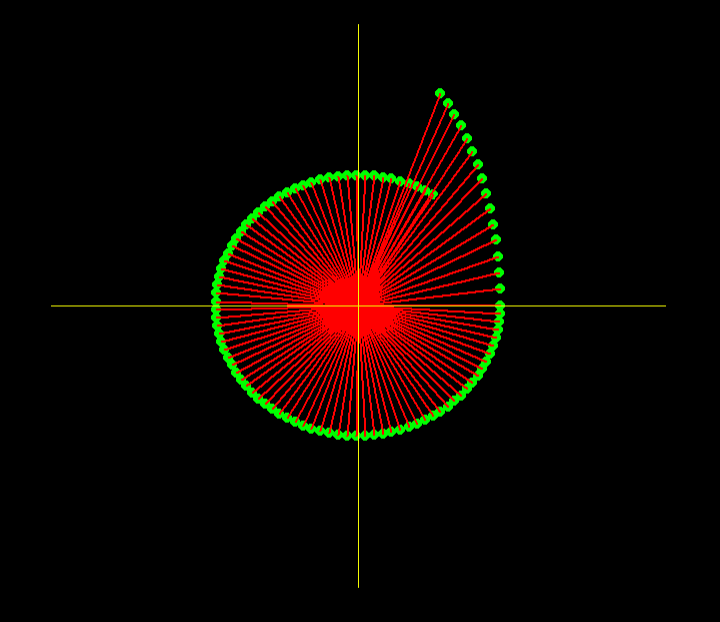
\includegraphics[scale=0.2]{02} & 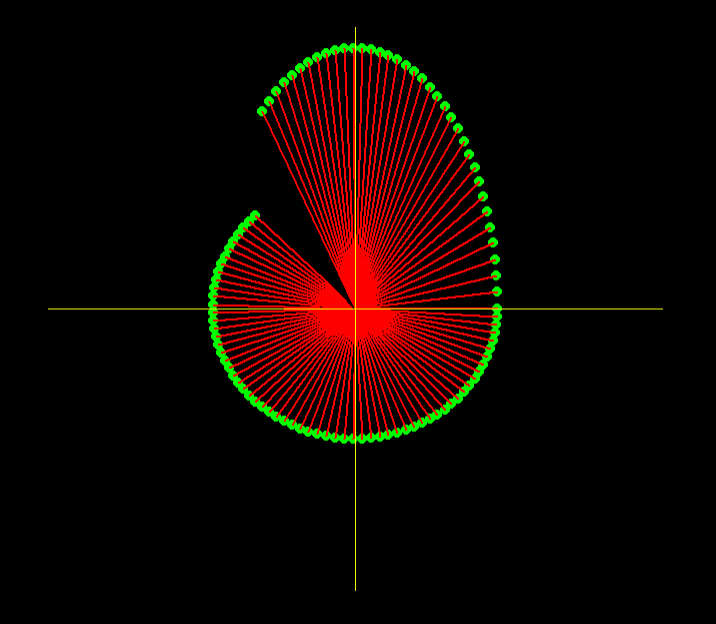
\includegraphics[scale=0.2]{03} & 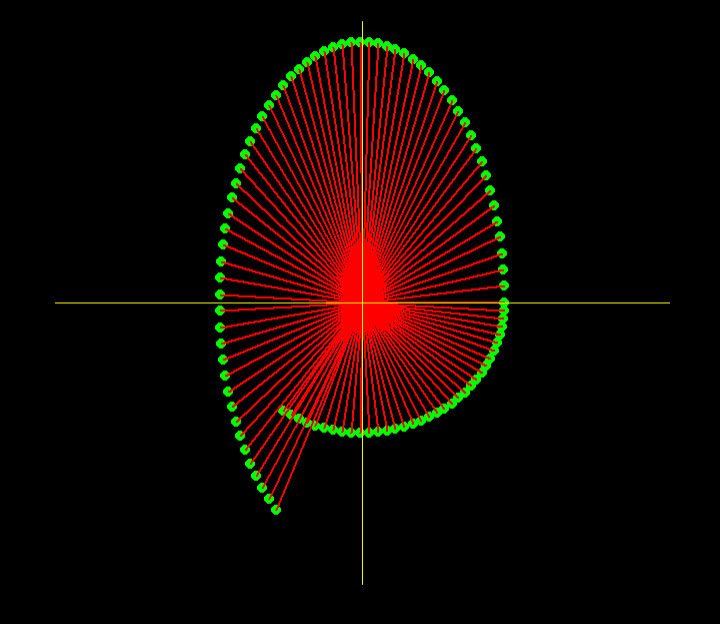
\includegraphics[scale=0.2]{04} 

\end{tabular}
\end{center}
\end{table}

\newpage

\begin{table}[h]

\begin{center}
\begin{tabular}{cc}

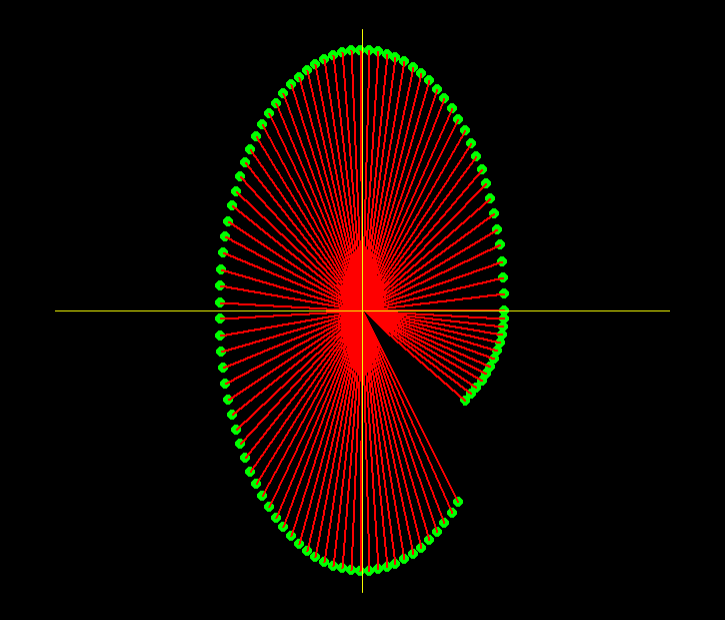
\includegraphics[scale=0.2]{05} & 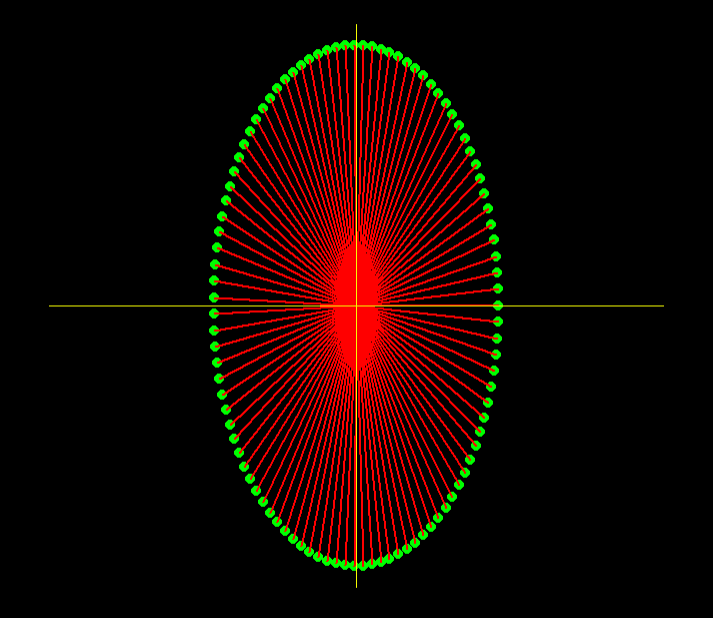
\includegraphics[scale=0.2]{06} 

\end{tabular}
\end{center}
\end{table}


\smallpencil \hspace{0.2cm} \textcolor{col2}{\textbf{\textit{Rotating}}} : Pre-multiplying any vector $ \begin{bmatrix} a \\ b \end{bmatrix} $ $\in$ $\mathbb{R}^2$ by 
  $ \begin{bmatrix} 
      \cos \theta & - \sin \theta \\
      \sin \theta & \cos \theta
    \end{bmatrix} $ rotates the vector by an angle $\theta$ anti-clockwise. Here we take $\theta = \dfrac{\pi}{4}$ and rotate the above vectors by $45^{\circ}$ anti-clockwise. \\
    
\faArrowAltCircleRight[regular] \textcolor{col1}{\textbf{\textit{Visualization}}} : \href{https://github.com/sakunisgithub/R-programming/blob/master/msc_sem_1_practicals/mahaveer_sir_assignments/assignment_04/transformation_3.R}{\textcolor{blue}{\textbf{Program to create the following animation is here.}}}

\begin{table}[h]

\begin{center}
\begin{tabular}{ccc}

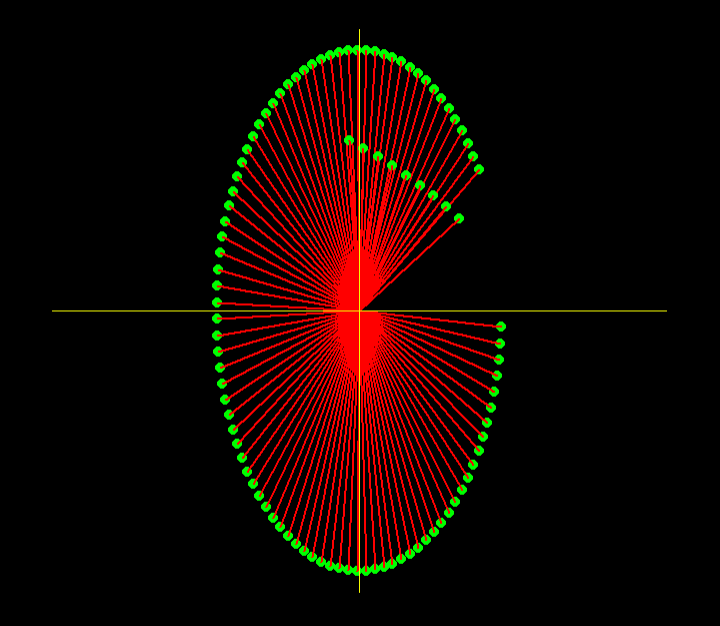
\includegraphics[scale=0.2]{07} & 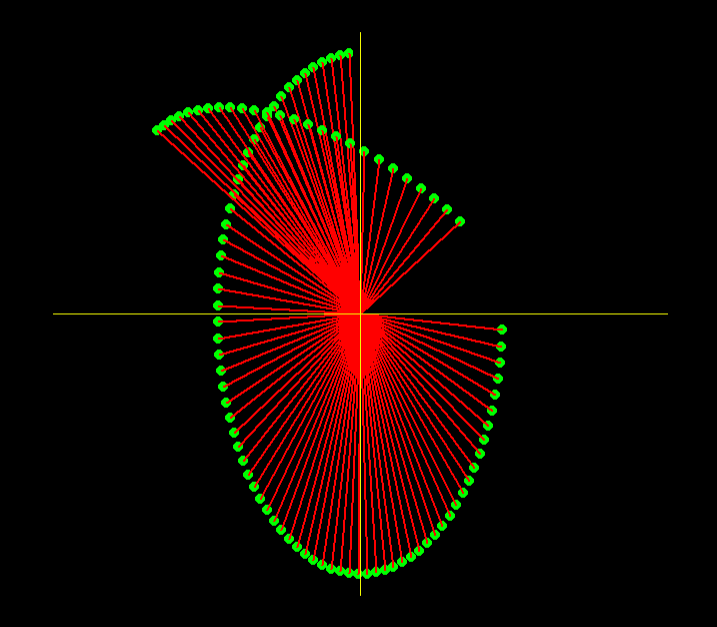
\includegraphics[scale=0.2]{08} & 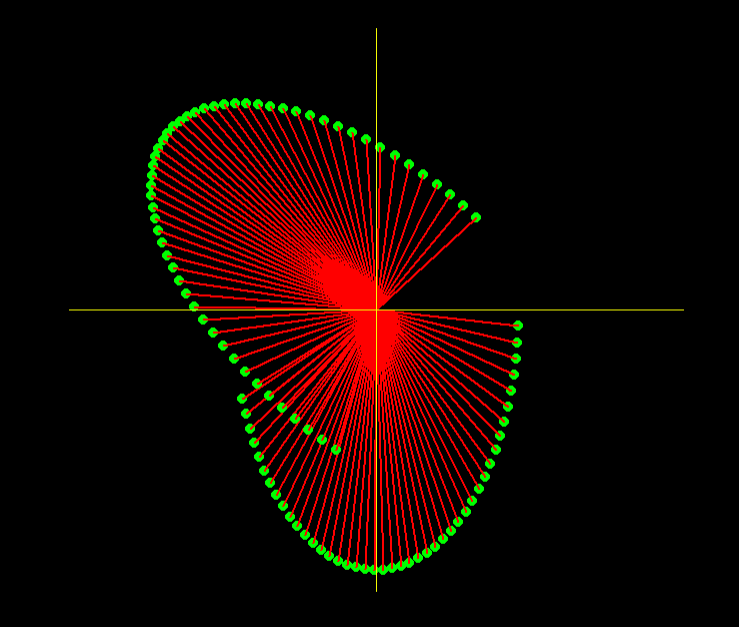
\includegraphics[scale=0.2]{09} 

\end{tabular}
\end{center}
\end{table}

\begin{table}[h]

\begin{center}
\begin{tabular}{cc}

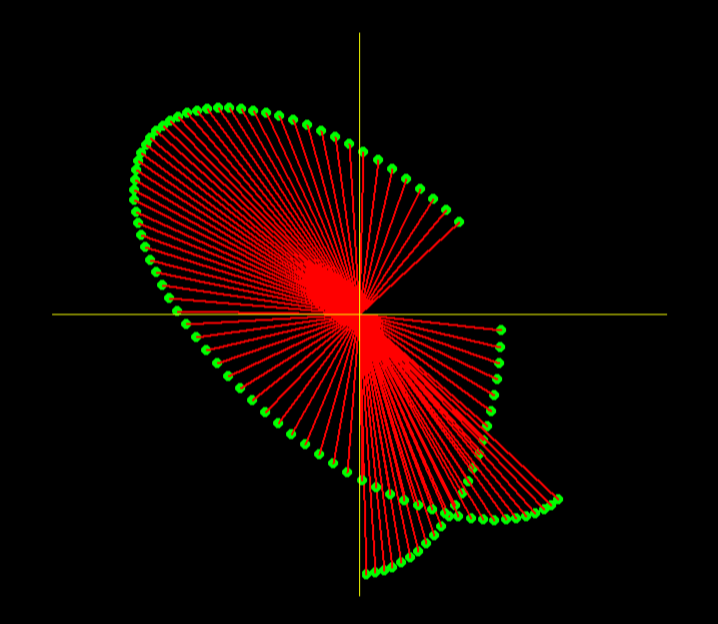
\includegraphics[scale=0.2]{10} & 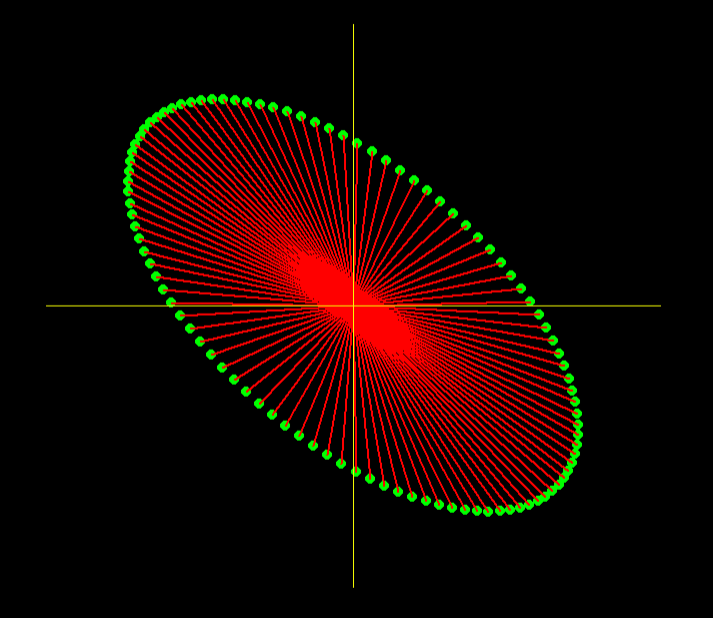
\includegraphics[scale=0.2]{11} 

\end{tabular}
\end{center}
\end{table}


\smallpencil \hspace{0.2cm} \textcolor{col2}{\textbf{\textit{Composition of Transformation}}} : Multiplication of two matrices results in a matrix that represents the combination of their transformations. Above we first stretched the 100 vectors two times along $y-$axis and then rotated them $45^{\circ}$ anti-clockwise. We can achieve the same by just pre-multiplying all the vectors by
	\begin{gather*} 
	  \begin{bmatrix} 
      	\cos \theta & - \sin \theta \\
	      \sin \theta & \cos \theta
    	  \end{bmatrix}_{\theta = \dfrac{\pi}{4}}
    	  	 \cdot 
	  \begin{bmatrix} 
	      1 & 0 \\
      	0 & 2 
        \end{bmatrix}         
        =         
        \begin{bmatrix}
        	0.7071068 & -1.414214 \\
        	0.7071068 & 1.414214
        \end{bmatrix}
      \end{gather*}

\faArrowAltCircleRight[regular] \textcolor{col1}{\textbf{\textit{Visualization}}} : \href{https://github.com/sakunisgithub/R-programming/blob/master/msc_sem_1_practicals/mahaveer_sir_assignments/assignment_04/transformation_4.R}{\textcolor{blue}{\textbf{Program to create the following animation is here.}}}

\begin{table}[!htbp]

\begin{center}
\begin{tabular}{ccc}

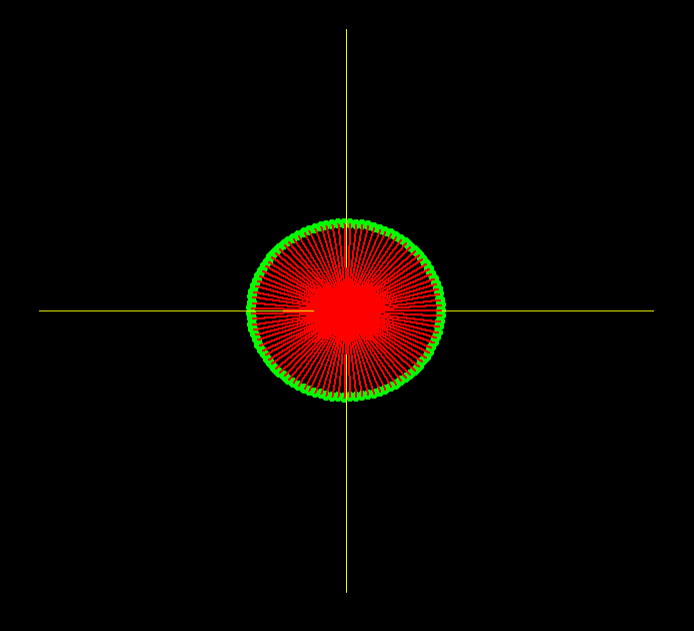
\includegraphics[scale=0.2]{12} & 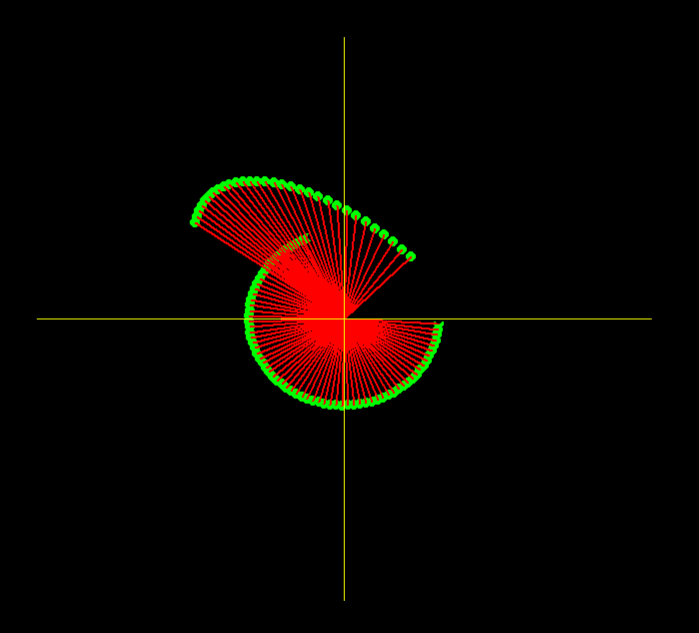
\includegraphics[scale=0.2]{13} & 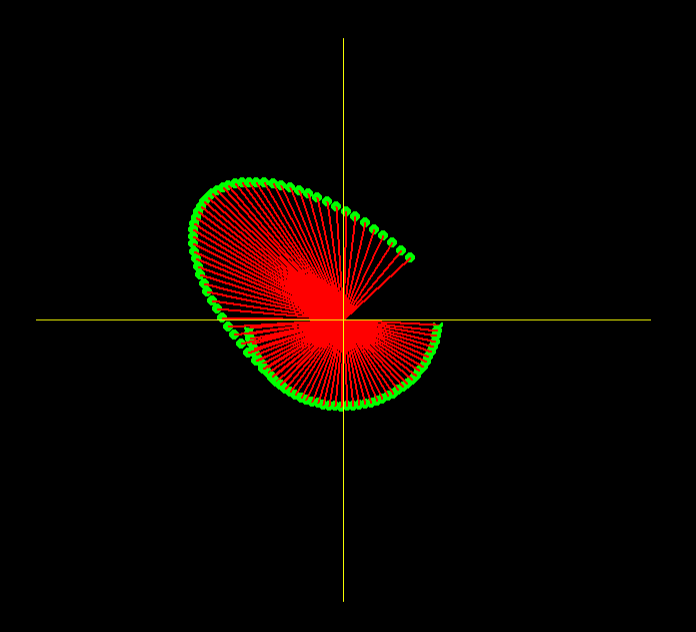
\includegraphics[scale=0.2]{14} 

\end{tabular}
\end{center}
\end{table}

\newpage

\begin{table}[h]

\begin{center}
\begin{tabular}{cc}

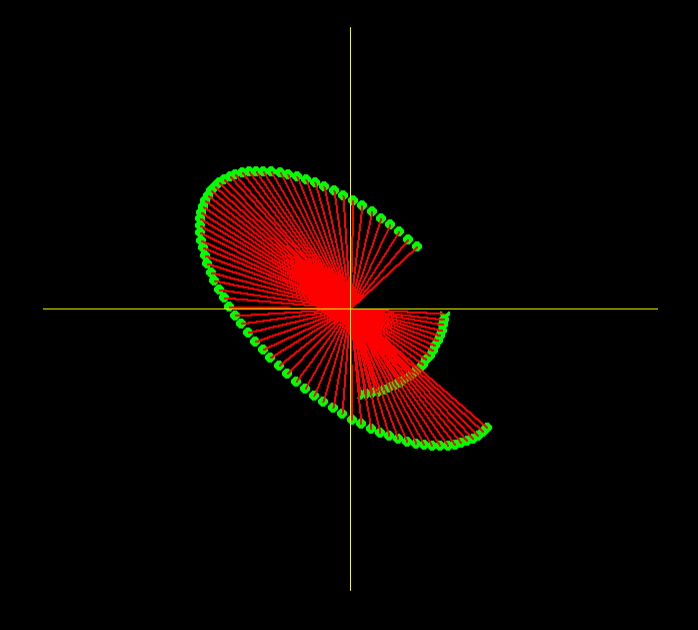
\includegraphics[scale=0.2]{15} & 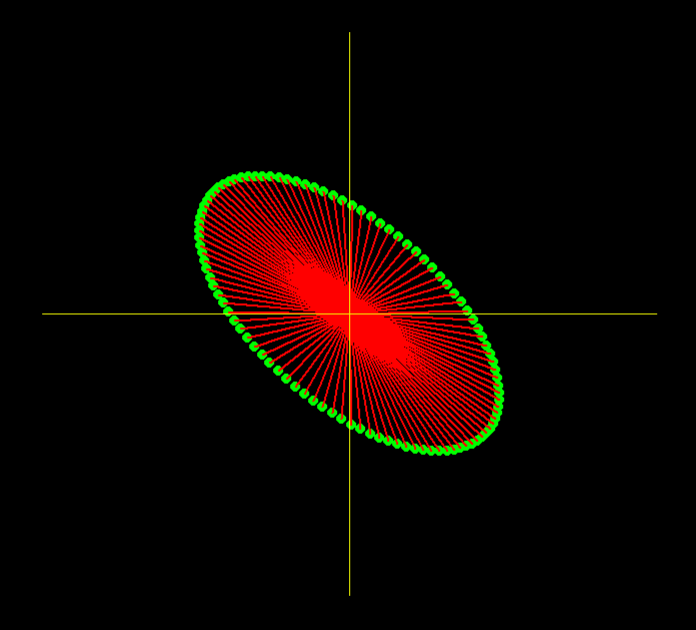
\includegraphics[scale=0.2]{16} 

\end{tabular}
\end{center}
\end{table}


\smallpencil \hspace{0.2cm} \textcolor{col2}{\textbf{\textit{Vector Spaces and Dimension}}} : Multiplying all the vectors of a vector space by a matrix of rank $r$ creates a new vector space of dimension $r$. Here we pre-multiply all the 100 vectors by 
	$ \begin{bmatrix} 
		1 & 1 \\
		1 & 1
	\end{bmatrix} $ which has rank 1 and see how $\mathbb{R}^2$ reduces to a straight line only. \\
	
\faArrowAltCircleRight[regular] \textcolor{col1}{\textbf{\textit{Visualization}}} : \href{https://github.com/sakunisgithub/R-programming/blob/master/msc_sem_1_practicals/mahaveer_sir_assignments/assignment_04/transformation_5.R}{\textcolor{blue}{\textbf{Program to create the following animation is here.}}}

\begin{table}[!htbp]

\begin{center}
\begin{tabular}{ccc}

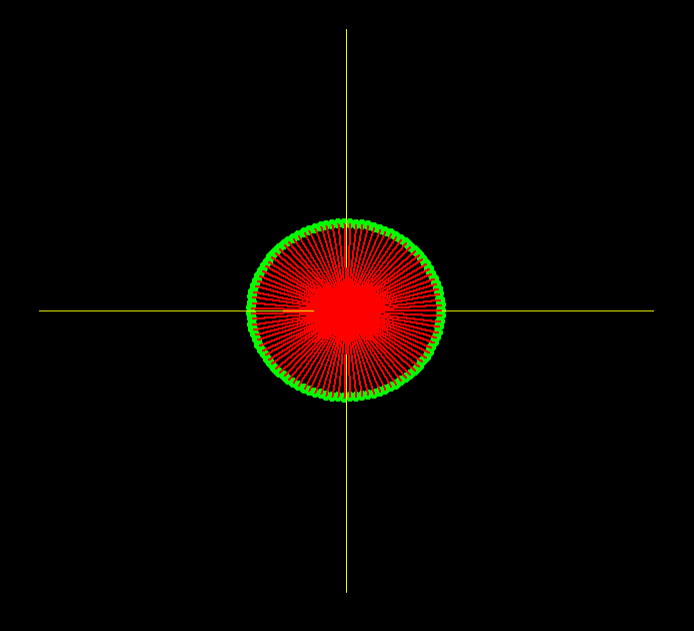
\includegraphics[scale=0.2]{17} & 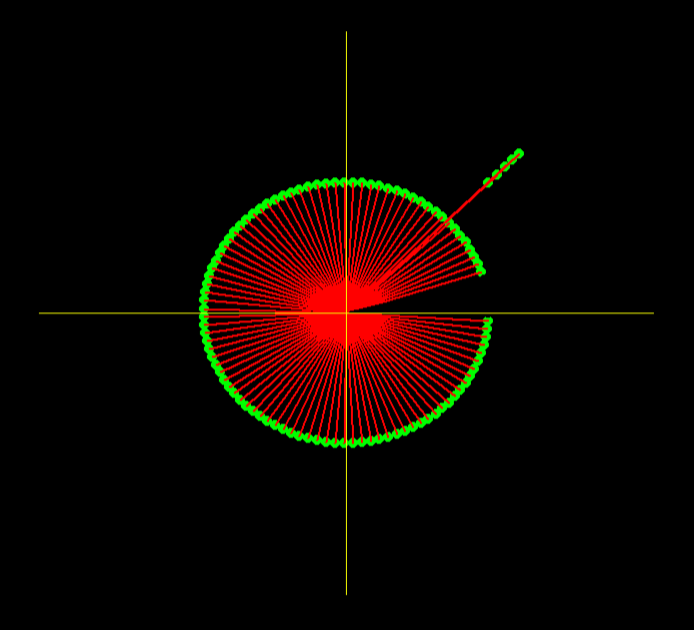
\includegraphics[scale=0.2]{18} & 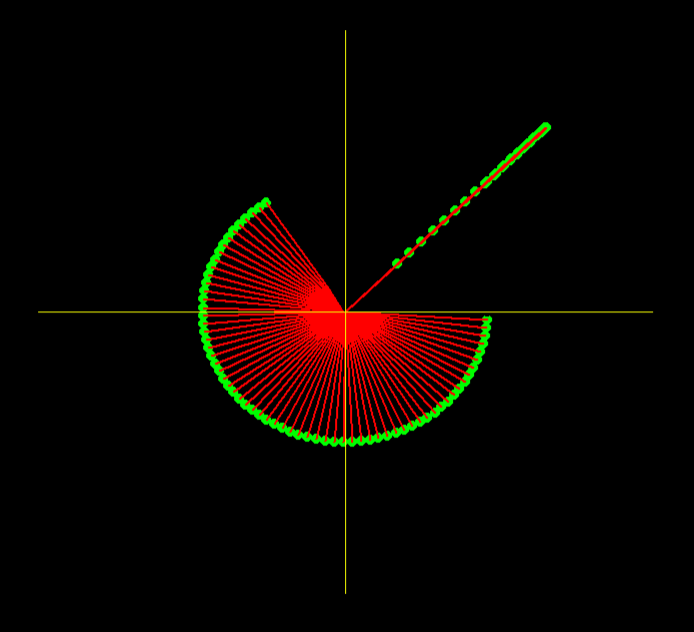
\includegraphics[scale=0.2]{19} \\

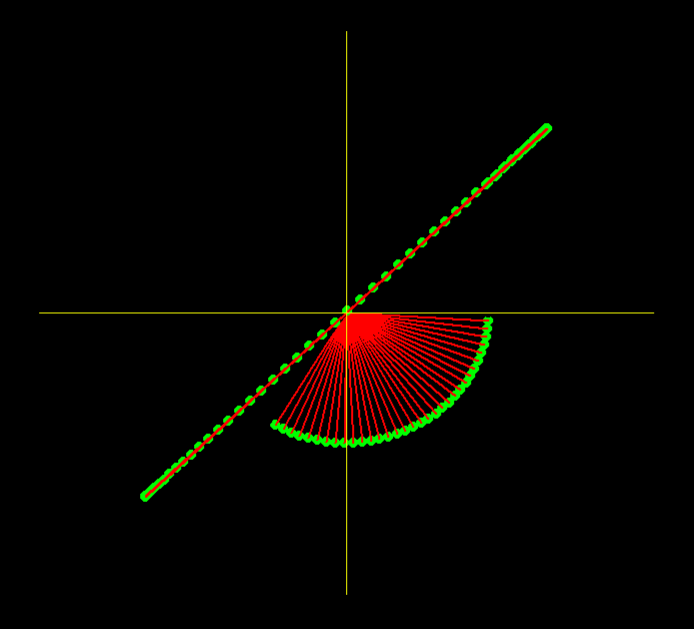
\includegraphics[scale=0.2]{20} & 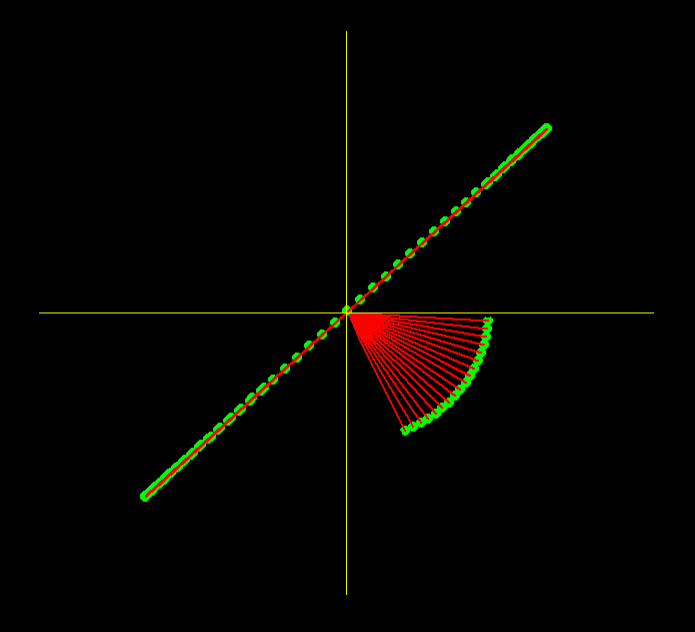
\includegraphics[scale=0.2]{21} & 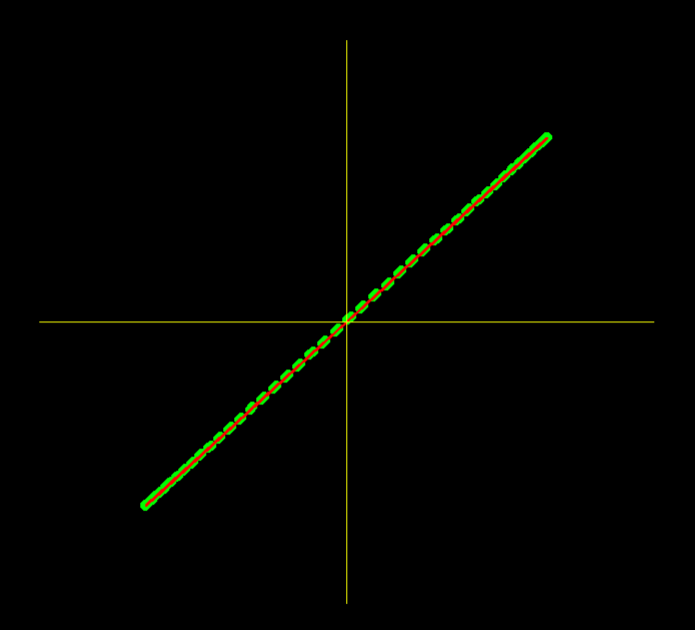
\includegraphics[scale=0.2]{22} \\


\end{tabular}
\end{center}
\end{table}


\smallpencil \hspace{0.2cm} \textcolor{col2}{\textbf{\textit{Eigenvectors and Eigenvalues}}} : Eigenvectors are those special vectors that, under the linear transformation defined by a matrix, remain within their own span, being scaled by a value, positive or negative depending on change of direction, called corresponding eigenvalues. \\
	
\hspace{0.5cm} In the \textcolor{col2}{\textbf{\textit{Scaling}}} example, observe that the vectors $\begin{bmatrix}
1 \\ 0
\end{bmatrix} $ and
$ \begin{bmatrix}
0 \\ 1
\end{bmatrix} $ get transformed to 
$\begin{bmatrix}
1 \\ 0
\end{bmatrix} $ and
$ \begin{bmatrix}
0 \\ 2
\end{bmatrix} $ respectively but remain in their corresponding spans only. This makes 
$\begin{bmatrix}
1 \\ 0
\end{bmatrix} $ and
$ \begin{bmatrix}
0 \\ 1
\end{bmatrix} $ eigenvectors of 
$ \begin{bmatrix} 
      1 & 0 \\
      0 & 2 
    \end{bmatrix} $ with corresponding eigenvalues 1 and 2. \\
    
\faArrowAltCircleRight[regular] \textcolor{col1}{\textbf{\textit{Visualization}}} : 

\begin{table}[!htbp]

\begin{center}
\begin{tabular}{cc}

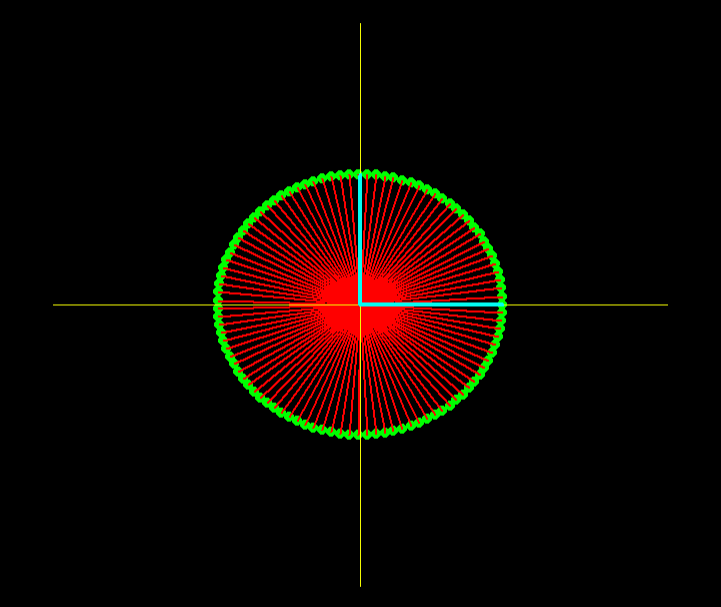
\includegraphics[scale=0.25]{23} &
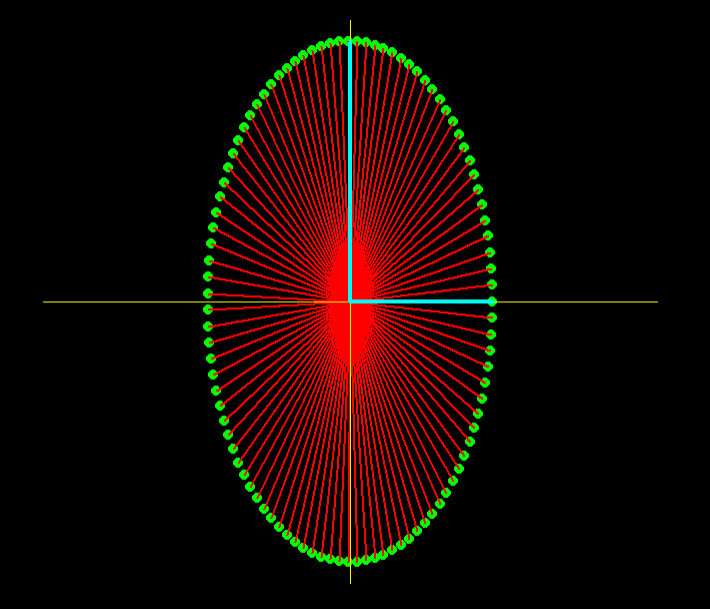
\includegraphics[scale=0.25]{24}

\end{tabular}
\end{center}

\end{table}




\end{document}